\documentclass[a4paper,12pt,twoside]{article}

\usepackage[utf8]{inputenc}
\usepackage[pdftex]{graphicx}
\usepackage{polski}
\usepackage{amsfonts}
\usepackage{verbatim}
\usepackage{indentfirst}
\usepackage{listings}
\usepackage{color}
\usepackage{tabto}
\newcommand{\TODO}{\textbf{TODO}}


% wyroznienie slow kluczowych
\newcommand{\tech}{\texttt}

%nazwy programow w tekscie -zuz
\newcommand{\prog}{\texttt}
%nazwy miar-jakosci -zuz
\newcommand{\qm}{\textit}
%wielowyrazowe nazwy ktore trzeba wyroznic 
\newcommand{\name}{\textsl}

\def\notka#1{\marginpar{\tiny\bf (#1)}}
%\def\notka#1{\relax}

\lstset{
language=C,
numbers=left,
frame = single, %lines - do lini gora-dol
breaklines=true, 
literate={:=}{{$\gets$}}1 {<=}{{$\leq$}}1 {>=}{{$\geq$}}1 {<>}{{$\neq$}}1,
emph={[1]foreach, end, procedure, is, in},emphstyle={[1]\textbf},
emph={[2]markSubdNodes, renumberNodes, createNewMesh, joinResultNodes, joinResultElements, getBoundaryNodes, createListOfFaces, sortNodesInFaces, sortFaces}, emphstyle={[2]\textsl}
}
\definecolor{light-gray}{gray}{0.985}
\definecolor{dark-gray}{gray}{0.10}
\lstnewenvironment{code}{\lstset{language=c,basicstyle=\ttfamily\scriptsize,numbers=right, numbersep=-20pt, xleftmargin=3pt,xrightmargin=3pt, stepnumber=1,breaklines=true,keywordstyle=\color{black},
stringstyle=\color{black},commentstyle=\color{dark-gray}\slshape,frame=single,backgroundcolor=\color{light-gray},  }}{}
\lstset{language=c,basicstyle=\ttfamily\scriptsize,numbers=right, numbersep=-20pt, xleftmargin=3pt,xrightmargin=3pt, stepnumber=1,breaklines=true,keywordstyle=\color{black},
stringstyle=\color{black},commentstyle=\color{dark-gray}\slshape,frame=single,backgroundcolor=\color{light-gray}}


% To trzeba wypelnic swoimi danymi
\title{Języki i Metody Programowania 2 projekt I:\\Automat Komórkowy}

\author{Patryk Milewski \\Paweł Zarczuk }


\begin{document}
\maketitle

\section{Specyfikacja funkcjonalna}

\subsection{Przeznaczenie}

Program przeprowadza symulację Gry w życie Johna Conwaya w siatce dwuwymiarowej wykorzystując dwa rodzaje sąsiedztwa(Moore oraz von Neumanna). Generuje obrazy poszczególnych generacji w postaci plików PNG oraz zapisuje ostatnią generację w postaci postaci pliku, który program może później wczytać.

\subsection{Funkcjonalność}
Działanie poszczególnych funkcjonalności uzależnione jest od parametrów, z którymi uruchamiany jest program oraz wartości ustawionych w pliku konfiguracyjnym.

Program oferuje dwie opcje wyboru początkowej generacji: wczytanie początkowej konfiguracji z pliku(z rozszerzeniem  .life) lub wygenerowanie losowej konfiguracji o wymiarach ustawionych w pliku konfiguracyjnym). Aby wybrać pierwszą z tych opcji, należy przy uruchamianiu programu podać odpowiedni parametr.
 
Ponadto umożliwia generowanie ustalonej przez użytkownika liczby generacji N, które standardowo zdefiniowane są w pliku konfiguracyjnym, lecz mogą zostać zmienione poprzez podanie odpowiedniego parametru programu z liczbą generacji N.

Umożliwia ustawienie zachowania się programu na brzegach. Dostępne są następujące opcje: brzegi puste, brzegi pełne, brzegi naprzemienne.

Program generuje N+1 obrazów przedstawiających generację początkową i  kolejne N generacji, a następnie zapisuje je w postaci pliku formacie PNG, o ustalonym przez użytkownika rozmiarze komórek(w pikselach) w folderze o nazwie podanej przy uruchamianiu programu. 

Dla ostatniej generacji program generuje plik .life, który zawiera opis bieżącej generacji(który może zostać potem wczytany). Jest on również zapisywany w folderze o nazwie podanej przy uruchamianiu programu.

\subsection{Wywołanie}

Program wywołujemy pisząc:
\medskip

   \quad \prog{Life.exe [opcja]...} 

   gdzie dopuszczalne opcje to:

\begin{description}
\item[\prog{ -w }] Nazwa katalogu do zapisu wyników


\item[\prog{ [-l ]}] (Opcjonalnie) nazwa pliku z siatką zerowej generacji,

\item[\prog{ [-g ]}] (Opcjonalnie) liczb generacji do wygenerowania (nie może być większa niż 999)
  
\end{description}

\subsection{Dane wejściowe}


   \verb+Plik tekstowy+ z rozszerzeniem .life, o postaci
\begin{verbatim}
n
c11 c12 c13 c14 ...
c21 c22 c23 c24 ...
... 
\end{verbatim} 
   gdzie:
   
    \verb+n+ to wymiary generowanej siatki n x n,
    
    \verb+c+ to cyfry 1, 0 oznaczające martwe(0)i żywe(1) komórki.\\
   Separatorem kolejnych komórek w linii jest spacja.
  
   \verb+Plik konfiguracyjny+ znajdujący się w katalogu z programem: life.conf. \\
   Struktura pliku konfiguracyjnego: 
  \begin{center}  
   [nazwaOpcji] = [wartość] 
  \end{center}
  
  Opis poszczególnych parametrów: \\  
  \prog{ neighborhoodSettings } 
  
  \hspace{1.5cm} Ustawienia sąsiedztwa: dla wartości 0 przyjmuje sąsiedztwo Von Neumann'a, a dla wartości 1 przyjmuje sąsiedztwo Moore'a
  
  \prog{ defaultBoardSize } 
  
  \hspace{1.5cm} Ustawienia wielkości planszy(uzywane tylko w przypadku losowego generowania komórek)  
  
  \prog{ edgeSettings } 
  
  \hspace{1.5cm} Ustawienie brzegów planszy, przyjmuje wartość 0- dla pustych brzegów, 1- dla pełnych brzegów, 2- dla brzegów naprzemiennych.
  
  \prog{ defaultGenerationCount } 
  
  \hspace{1.5cm}  Domyślna liczba generowanych generacji. Liczba generacji nie może być większa niż 999.
  
  \prog{ cellSize } 
  
  \hspace{1.5cm}  Wielkość pojedynczej komórki na obrazie PNG generacji (w pikselach)
   


\subsection{Format wyników}

   Plik o rozszerzeniu .life o takiej samej strukturze jak dane wejściowe oraz N+1 obrazów generacji w formacie png.



\section{Architektura kodu}
Program składa się z 5 modułów: main, gameOperator, boardGenerator, gameSettings, pngOperator.

  W module main znajdują się głównie wywołania funkcji, w module gameOperator znajdują się najważniejsze funkcje programu, odpowiedzialne za symulację poszczególnych generacji. boardGenerator to moduł zawierający dwie funkcje służące do generowania planszy. GameSettings to moduł zawierający obsługę pliku konfiguracyjnego, zaś pngOperator służy do tworzenia plików PNG.
  
   \prog{main} 
  
  \hspace{1.5cm}W module tym znajdują się wywołania poszczególnych funkcji, wczytywanie parametrów uruchomienia programu oraz obsługa wypisywania informacji o błędach.

  \prog{gameOperator} 

  \hspace{1.5cm} Moduł składający się z funkcji createBoard - która w zależności od podanych parametrów decyduje czy generować losową planszę czy wczytać planszę z pliku; funkcji gameSimulation, która jest odpowiedzialna za podstawową funkcjonalność programu. Odpowiada ona za symulację kolejnych generacji, wykorzystując do tego funkcje checkAlive, checkCellMooreNeighborhood, checkCellVonNeumannNeighborhood, findFileName(również zawarte w tym module - są opisane poniżej). Najważniejszym elementem tej funkcji są dwie pętle wykonywane dla każdej generacji oraz funkcje zapisującą dane w postaci obrazu PNG - printFile:
  \begin{lstlisting}
        for (int i = 1; i < boardSize - 1; i++)      // i=1 and, i < boardSize-1, cause cells are stored from index 1 to 
            for (int j = 1; j < boardSize - 1; j++){ // index equal boardSize-1, other space is designed for border
                int aliveNeighbours;
                if (settings.neighborhoodSettings == 1)
                    aliveNeighbours = checkCellMooreNeighborhood(gameBoard->fields, i, j);
                else
                    aliveNeighbours = checkCellVonNeumannNeighborhood(gameBoard->fields, i, j);
                newFields[i][j]=checkAlive(aliveNeighbours,gameBoard->fields[i][j]);
            }
        freeFields(gameBoard); //Free old generation array
        gameBoard->fields=newFields; //puts new generation into struct gameBoard
        findFileName(saveName,l+1,fileName);
        errorCommand=printFile(fileName, gameBoard,settings.cellSize); // generate visualization of generation in PNG format
\end{lstlisting}
Funkcja checkAlive sprawdza czy komórka powinna zmienić swój stan  z żywej na martwą lub odwrotnie, w zależności od liczby komórek żywych.
Funkcje checkCellMooreNeighborhood i checkCellVonNeumannNeighborhood służą do zliczania żywych komórek według zasad odpowiedniego sąsiedztwa.
Funkcja findFileName znajduje nazwy dla kolejnych obrazów PNG.
Do modułu tego należy także struktura gameBoard\_t :
\begin{lstlisting}
typedef struct gameBoard{
    int boardSize;
    short **fields;
}   gameBoard_t;
\end{lstlisting}
  \prog{boardGenerator} 

  \hspace{1.5cm} Moduł składający się z funkcji boardGenerator - służącej do generowania losowej mapy, oraz z funkcji setBorders służącej do tworzenia brzegów według ustawień.

  \prog{gameSettings} 

  \hspace{1.5cm} Moduł składający się z funkcji służącej do wczytywania zawartości pliku konfiguracyjnego do struktury settings typu gameSettings\_t:

\begin{lstlisting}
typedef struct gameSettings{
    int defaultBoardSize;
    int neighborhoodSettings;
    int edgeSettings;
    int isBoardLoaded;
    int cellSize;
    int defaultGenerationCount;
} gameSettings_t;
\end{lstlisting}

  \prog{pngOperator} 

  \hspace{1.5cm} Moduł składający się z funkcji służącej do generowania z informacji o planszy zawartych w strukturze gameBoard\_t obrazów w formacie PNG o wielkosci poszczególnych komórek pobranych ze struktury typu gameSettings\_t.

\section{Testy}

Test I: 
Test 
  \begin{center}
\begin{lstlisting}
18
0 0 0 0 0 0 0 0 0 0 0 0 0 0 0 0 0 0  
0 0 0 0 0 0 0 0 0 0 0 0 0 0 0 0 0 0  
0 0 0 0 0 0 0 0 0 0 0 0 0 0 0 0 0 0  
0 0 0 0 0 0 0 0 0 0 0 0 0 0 0 0 0 0  
0 0 0 0 0 0 0 0 0 0 0 0 0 0 0 0 0 0 
0 0 0 0 0 0 0 0 1 1 0 0 0 0 0 0 0 0  
0 0 0 0 0 0 1 0 0 0 0 1 0 0 0 0 0 0 
0 0 0 0 0 1 0 0 0 0 0 0 1 0 0 0 0 0
0 0 0 0 1 0 0 0 0 0 0 0 0 1 0 0 0 0  
0 0 0 0 1 0 0 0 0 0 0 0 0 1 0 0 0 0  
0 0 0 0 1 0 0 0 0 0 0 0 0 1 0 0 0 0  
0 0 0 0 0 1 0 0 0 0 0 0 1 0 0 0 0 0  
0 0 0 0 0 0 1 0 0 0 0 1 0 0 0 0 0 0  
0 0 0 0 0 0 0 0 1 1 0 0 0 0 0 0 0 0  
0 0 0 0 0 0 0 0 0 0 0 0 0 0 0 0 0 0 
0 0 0 0 0 0 0 0 0 0 0 0 0 0 0 0 0 0 
0 0 0 0 0 0 0 0 0 0 0 0 0 0 0 0 0 0 
0 0 0 0 0 0 0 0 0 0 0 0 0 0 0 0 0 0 
0 0 0 0 0 0 0 0 0 0 0 0 0 0 0 0 0 0
0 0 0 0 0 0 0 0 0 0 0 0 0 0 0 0 0 0

\end{lstlisting}
  \end{center}
\begin{figure}[htb]
  % wyśrodkowanie zawartości pola obrazka
  \begin{center}
      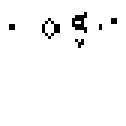
\includegraphics[width=.75\textwidth]{test1.png}
      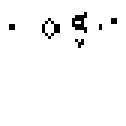
\includegraphics[width=.75\textwidth]{test1.png}
      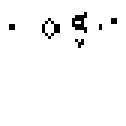
\includegraphics[width=.75\textwidth]{test1.png}
      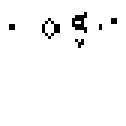
\includegraphics[width=.75\textwidth]{test1.png}
      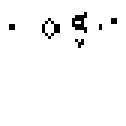
\includegraphics[width=.75\textwidth]{test1.png}
      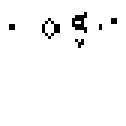
\includegraphics[width=.75\textwidth]{test1.png}
      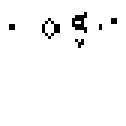
\includegraphics[width=.75\textwidth]{test1.png}
      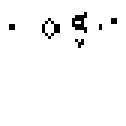
\includegraphics[width=.75\textwidth]{test1.png}
      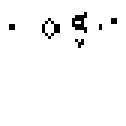
\includegraphics[width=.75\textwidth]{test1.png}
    \caption{Poglądowa architektura systemu RaSS}
    % etykieta obrazka umożliwia odwołanie się do niego w tekście
    \label{RaSS}
  \end{center}
\end{figure}

\end{document}
